\documentclass[a4paper,11pt,titlepage]{scrbook}
\usepackage[utf8]{inputenc}
\usepackage[spanish]{babel}

% \usepackage[style=list, number=none]{glossary} %si se va a usar glosario, quitar marca de comentario
%\usepackage{titlesec}
%\usepackage{palatino} %usar fot palatino en vez de times roman

%\decimalpoint %revisar
%\usepackage{dcolumn} %revisat
%\newcolumntype{.}{D{.}{\esperiod}{-1}}
%\makeatletter
%\addto\shorthandsspanish{\let\esperiod\es@period@code}
%\makeatother


%\usepackage[chapter]{algorithm}
%\RequirePackage{verbatim}
%\RequirePackage[Glenn]{fncychap}
\usepackage{fancyhdr}
\usepackage{graphicx}
\usepackage{afterpage}
\usepackage{longtable}
\usepackage{xcolor}
\definecolor{portada}{RGB}{239,206,53}
\definecolor{base}{RGB}{35,31,32}
\usepackage{pdfpages}

\usepackage[backend=bibtex,style=verbose-trad2]{biblatex} % Use biblatex package
%\bibliographystyle{apalike}
\bibliography{bibliografia/bibliografia} % The name of the .bib file (name without .bib)
%%\nocite{*} %incluye TODOS los documentos de la base de datos bibliográfica sean o no citados en el texto
%\bibliography{bibliografia/bibliografia}\addcontentsline{toc}{chapter}{Bibliografía} %sustituir bibliografía con el nombre del fichero bibtex con la bibliografía


%Instrucciones para poder escribir código y mostrarlo de manera elegante:
\definecolor{gray97}{gray}{.97}
\definecolor{gray75}{gray}{.75}
\definecolor{gray45}{gray}{.45}
\definecolor{gray30}{gray}{.94}

\usepackage{listings}
\lstset{ frame=Ltb,
framerule=0pt,
aboveskip=0.5cm,
framextopmargin=3pt,
framexbottommargin=3pt,
framexleftmargin=0.4cm,
framesep=0pt,
rulesep=.4pt,
backgroundcolor=\color{gray97},
rulesepcolor=\color{black},
%
stringstyle=\ttfamily,
showstringspaces = false,
basicstyle=\small\ttfamily,
commentstyle=\color{gray45},
keywordstyle=\bfseries,
%
numbers=left,
numbersep=15pt,
numberstyle=\tiny,
numberfirstline = false,
breaklines=true,
literate={á}{{\'a}}1 {Á}{{\'A}}1 {é}{{\'e}}1 {É}{{\'e}}1 {í}{{\'i}}1  {Í}{{\'I}}1  {ó}{{\'o}}1  {Ó}{{\'O}}1  {ú}{{\'u}}1  {Ú}{{\'U}}1  {Ñ}{{\~N}}1 {ñ}{{\~n}}1 ,
}



% minimizar fragmentado de listados
\lstnewenvironment{listing}[1][]
   {\lstset{#1}\pagebreak[0]}{\pagebreak[0]}

\lstdefinestyle{Consola}
   {basicstyle=\scriptsize\bf\ttfamily,
    backgroundcolor=\color{gray30},
    frame=single,
    numbers=none
   }
\lstdefinestyle{C}
	{basicstyle=\scriptsize,
	frame=single,
	language=C,
	numbers=left
	}
\lstdefinestyle{CodigoC++}
        {basicstyle=\small,
	frame=single,
	backgroundcolor=\color{gray30},
	language=C++,
	numbers=left
 	}
\lstdefinestyle{PHP}
	{basicstyle=\scriptsize,
%        {basicstyle=\small,
	frame=single,
	language=PHP,
	numbers=left
	}
	



% ********************************************************************
% Información sobre el TFG. Comentar lo que NO se desee añadir y sustituir con la información correcta.
% ********************************************************************
\newcommand{\myTitle}{Título del Trabajo de Fin de Grado}
\newcommand{\mySubtitle}{Subtítulo del proyecto}
\newcommand{\myDegree}{Grado en Ingeniería Multimedia}
\newcommand{\myName}{Nombre Apellido1 Apellido2 (alumno)}
\newcommand{\myProf}{Nombre Apellido1 Apellido2 (tutor1)}
\newcommand{\myOtherProf}{Nombre Apellido1 Apellido2 (tutor2)}
\newcommand{\myFaculty}{Escuela Politécnica Superior de la Universidad de Alicante}
\newcommand{\myFacultyShort}{EPS UA}
\newcommand{\depTutorOne}{Departamento del tutor}
\newcommand{\depTutorTwo}{Departamento del cotutor}


\newcommand{\myUni}{\protect{Universidad de Alicante}}
\newcommand{\myLocation}{Alicante}
\newcommand{\myTime}{\today}
%\newcommand{\myVersion}{Version 0.1}

\newcommand{\logoGrado}{imagenes/logoim.jpg}
\newcommand{\logoFacultad}{imagenes/logoeps.jpg}
\newcommand{\logoUniversidad}{imagenes/logoua.jpg}

\usepackage{url}

% Definición de comandos que me son útiles:
%\renewcommand{\indexname}{Índice alfabético}
%\renewcommand{\glossaryname}{Glosario}

\pagestyle{fancy}
\fancyhf{}
\fancyhead[LO]{\leftmark}
\fancyhead[RE]{\rightmark}
\fancyhead[RO,LE]{\textbf{\thepage}}
\renewcommand{\chaptermark}[1]{\markboth{\textbf{#1}}{}}
\renewcommand{\sectionmark}[1]{\markright{\textbf{\thesection. #1}}}


\setlength{\headheight}{1.5\headheight}

\newcommand{\HRule}{\rule{\linewidth}{0.5mm}}
%Definimos los tipos teorema, ejemplo y definición podremos usar estos tipos
%simplemente poniendo \begin{teorema} \end{teorema} ...
\newtheorem{teorema}{Teorema}[chapter]
\newtheorem{ejemplo}{Ejemplo}[chapter]
\newtheorem{definicion}{Definición}[chapter]
 
\newcommand{\bigrule}{\titlerule[0.5mm]}


%Para conseguir que en las páginas en blanco no ponga cabeceras
\makeatletter
\def\clearpage{%
  \ifvmode
    \ifnum \@dbltopnum =\m@ne
      \ifdim \pagetotal <\topskip
        \hbox{}
      \fi
    \fi
  \fi
  \newpage
  \thispagestyle{empty}
  \write\m@ne{}
  \vbox{}
  \penalty -\@Mi
}
\makeatother

\usepackage[pdfborder={000}]{hyperref} %referencia
\hypersetup{
pdfauthor = {\myName (email (en) ua (punto) es)},
pdftitle = {\myTitle},
pdfsubject = {},
pdfkeywords = {palabra_clave1, palabra_clave2, palabra_clave3, ...},
pdfcreator = {LaTeX con el paquete ....},
pdfproducer = {pdflatex}
}
%AQUI COMIENZA LA LISTA DE FICHEROS A INCLUIR



\begin{document}
\renewcommand{\listtablename}{Índice de tablas} %para sustituir la palabra cuadro por tabla
\renewcommand{\tablename}{Tabla}
\renewcommand{\lstlistingname}{Listado}
\renewcommand{\lstlistlistingname}{Índice de \lstlistingname s}

\frontmatter
\begin{titlepage}

\newlength{\centeroffset}
\setlength{\centeroffset}{-0.5\oddsidemargin}
\addtolength{\centeroffset}{0.5\evensidemargin}
\thispagestyle{empty}

\includepdf[pages={1},pagecommand={},fitpaper=true,trim=0 0 0 0, 
offset=0 0,turn=true,noautoscale=true]{portada/portada.png}

\end{titlepage}
\pagecolor{white} %la portada en color
\begin{titlepage}
 
 
\setlength{\centeroffset}{-0.5\oddsidemargin}
\addtolength{\centeroffset}{0.5\evensidemargin}
\thispagestyle{empty}

\noindent\hspace*{\centeroffset}\begin{minipage}{\textwidth}

\centering


% Title

%{\Huge\bfseries Título del proyecto\\ }
{\Huge\bfseries \myTitle}

\noindent\rule[-1ex]{\textwidth}{3pt}\\[3.5ex]
{\large\bfseries \mySubtitle\\[4cm]}
\end{minipage}

\vspace{2.5cm}
\noindent\hspace*{\centeroffset}\begin{minipage}{\textwidth}
\centering

\textbf{Autor}\\ {\myName}\\[2.5ex]
\textbf{Directores}\\
{\normalsize \myProf\\
\small\textit \depTutorOne\\
\normalsize \myOtherProf\\
\small\textit \depTutorTwo\\[2cm]}

\includegraphics[scale=0.25]{\logoGrado}


\textsc{\myDegree}\\

\centering
\begin{minipage}[l]{7cm}
\includegraphics[width=5cm]{\logoFacultad}
\end{minipage}
\begin{minipage}[r]{7cm}
\includegraphics[width=5cm]{\logoUniversidad}
\end{minipage}


%\textsc{\myFaculty}\\

%\large\bfseries \textsc{\myUni}\\
ALICANTE, \myTime

\end{minipage}
%\addtolength{\textwidth}{\centeroffset}
\vspace{\stretch{2}}

\end{titlepage}


 %la portada en b/n
\chapter*{Preámbulo}
\thispagestyle{empty}
Poner aquí un texto breve que debe incluir entre otras:
\begin{quote}
``las razones que han llevado a la realización del estudio, el tema, la finalidad y el alcance y también los agradecimientos por las ayudas, por ejemplo apoyo económico (becas y subvenciones) y las consultas y discusiones con los tutores y colegas de trabajo. \cite{UNE50136:97}''
\end{quote}

\cleardoublepage %salta a nueva página impar
% Aquí va la dedicatoria si la hubiese. Si no, comentar la(s) linea(s) siguientes
\chapter*{}
\setlength{\leftmargin}{0.5\textwidth}
\setlength{\parsep}{0cm}
\addtolength{\topsep}{0.5cm}
\begin{flushright}
\small\em{
A mi esposa Marganit, y a mis hijos Ella Rose y Daniel Adams,\\
sin los cuales habría podido acabar este libro dos años antes \footnote{Dedicatoria de Joseph J. Roman en ``An Introduction to Algebraic Topology''}
}
\end{flushright}


\cleardoublepage %salta a nueva página impar
% Aquí va la cita célebre si la hubiese. Si no, comentar la(s) linea(s) siguientes
\chapter*{}
\setlength{\leftmargin}{0.5\textwidth}
\setlength{\parsep}{0cm}
\addtolength{\topsep}{0.5cm}
\begin{flushright}
\small\em{
Si consigo ver más lejos\\
es porque he conseguido auparme\\ 
a hombros de gigantes
}
\end{flushright}
\begin{flushright}
\small{
Isaac Newton.
}
\end{flushright}
\cleardoublepage %salta a nueva página impar
 %editar este texto (capitulos/preliminares.tex) para cambiar preámbulo, agradecimientos y dedicatorias
\tableofcontents
\listoffigures
\listoftables
\lstlistoflistings

\mainmatter %entre frontmatter y mainmatter, la numeración es en romanos.

%a continuación se propone un esquema de trabajo que puede ser alterado justificadamente.




\chapter{Introducción}

El 12 de octubre de 1492 un temerario explorador, Cristobal Colón, y su tripulación pisan la arena de una isla muy al oeste de Europa conocida como Guanahani. Este hecho marca un hito en la historia de la humanidad pues los cambios culturales, económicos, políticos y militares que produce dan lugar a la llamada Edad Moderna.\\
Colón vio una oportunidad de negocio en el control de las rutas comerciales que unían Europa con Asia pues eran recorridas por miles de comerciantes que traían especias y productos de lujo desde las tierras de Extremo Oriente. El comercio además se realizaba por tierra, lo que lo convertía en un proceso lento, inseguro e ineficiente, además de enriquecedor para los árabes que controlaban las rutas comerciales.

El proyecto tenía un gran interés económico pues como se ha dicho anteriormente, el control de una ruta comercial con Asia era muy lucrativo, pero a su vez tenía un gran riesgo ya que el futuro de la expedición era tremendamente incierto y había pocas posibilidades de encomendarse al vasto oceano y volver para contarlo. Debido a esta incertidumbre sobre el retorno de la inversión a Colón le fue complicado encontrar financiación para su proyecto, hasta que finalmente, tras recurrir a varios monarcas y mecenas,  los Reyes Católicos le proveyeron de los rescursos necesarios para iniciar su aventura.

Se podría considerar a Cristobal Colón como un emprendedor, a pesar de que el término fue usado por primera vez doscientos años después por el economista Richard Cantillon que define al emprendedor como ''La persona que paga un cierto precio para revender un producto a un precio incierto, por ende tomando decisiones acerca de la obtención y el uso de recursos, y admitiendo consecuentemente el riesgo en el emprendimiento" \cite[ pág 21]{ashokbhanudasnavale2013}.
De esta definición se puede apreciar que un emprendedor inicia proyectos y acepta la incertidumbre y el riesgo que ello conlleva, puesto que en caso de desastre es él quien carga con la responsabilidad.

La actitud emprendedora ha sido una constante a lo largo de la historia de la humanidad: desde Cristobal Colón hasta Bill Gates, pasando por Leonardo Da Vinci, Henry Ford o Nikola Tesla; hombres y mujeres con coraje han empezado proyectos bajo una idea prometedora y asumiendo grandes riesgos, motivados por la pasión y las perspectivas de éxito. 

El emprendimiento es una actividad especialmente necesaria para el progreso de una sociedad pues es un proceso que crea riqueza, innovación y empleo. Los emprendedores crean productos y servicios revolucionarios que hacen la vida de las personas más fácil, mejorando por ello su calidad de vida. Además suele ser una salida muy recurrida en épocas de crisis económicas debido a la escasez de empleo.

\section{Emprendimiento y el fenómeno startup}

Cada vez es más frecuente escuchar el término startup, pequeñas empresas dedicadas al ámbito tecnológico que alcanzan en pocos años grandes cuotas de mercado y se venden por millones de euros a empresas más grandes.

 El fenómeno goza de tanta popularidad que ha inspirado incluso a series como Silicon Valley, que narra las aventuras de un grupo de jóvenes ingenieros que crean una startup tecnológica y se enfrentan al reto de sobrevivir en un ecosistema hostil como es el mercado; la película Piratas de Silicon Valley, que narra la historia de enfrentamiento entre Microsoft y Apple; la película La red social que cuenta la historia de Mark Zuckerberg y como crea la red social Facebook.

Llegado a este punto cabe preguntarse: ¿Qué es exactamente una startup?. Es un error común pensar que las startup son simplemente versiones más pequeñas de empresas grandes. En palabras de los gurús del emprendimiento Steve Blank y Bob Dorf, ''Una startup es una organización temporal en busca de un modelo de negocio rentable, que pueda repetirse y que es escalable"\cite{steveblankbobdorf2013}.\\
De la anterior definición se puede extraer que una startup:
\begin{itemize}
	\item Es una organización temporal, es decir, el objetivo no es ser siempre una startup. El objetivo es convertirse en una empresa consolidada.
	\item No conoce con seguridad cual va a ser su actividad. En su lugar parten de un modelo de negocio temporal que va evolucionando a medida que interactúa con el mercado.
	\item Busca un modelo de negocio repetible y escalable, que le permita ejecutar dicho modelo de negocio durante un tiempo indefinido y además expandirse.
\end{itemize}
El emprendimiento es inherente al fenómeno startup pues la incertidumbre es un pilar fundamental al crear una de estas empresas, que ni siquiera tienen un modelo de negocio que se pueda asegurar que va a funcionar.

\section{Estado actual del emprendimiento en España}

Si bien el fenómeno startup nació en EEUU y es allí donde está más consolidado, en España es una tendencia igualmente extendida. Atendiendo a cifras de financiación ''en 2015, las startups españolas lograron financiación por valor de 500 millones de euros, un 87\%   más que en 2014, cuando apenas se invirtieron 286 millones de euros" \cite{albertoiglesiasfraga2016}.\\
Actualmente en nuestro país hay 1783 empresas emergentes distribuidas principalmente en Madrid, Cataluña y la Comunidad valenciana. Dichas empresas se dedican principalmente al ecommerce(22\%), social media(13\%) y las empresas(12\%). En cuanto a la financiación, 172 inversores operan en el ámbito startup a lo largo de la península \cite{startupxplore2017} y los fondos que han aportado crecen año a año: ''en 2013 tres startups lograron rondas de financiación que superaran los 10 millones de euros [...] en 2014, esta cifra aumentó a cuatro [...] el pasado año la explosión no tuvo parangón, ya que hasta 13 startups lograron capitalizar más de 10 millones de euros para fomentar su desarrollo" \cite{albertoiglesiasfraga2016}. 

\section{Lean startup}

Lean startup es un modelo de gestión empresarial dinámico ampliamente utilizado en la creación de empresas emergentes. En contraposición a las metodologías tradicionales, Lean startup se basa en ciclos de desarrollo cortos que permiten sacar el producto al mercado de forma temprana. De este modo se puede obtener retroalimentación de los clientes en las etapas iniciales de la empresa, lo que da lugar a que el producto cambia y se adapta a las necesidades de los clientes.

El primer paso para crear una startup según esta metodología es plasmar las hipótesis sobre el modelo de negocio en el Lean canvas \ref{leanCanvas}( como se cita la imagen????? http://innokabi.com/wp-content/uploads/2013/09/lienzo-lean-canvas-de-ash-maurya.jpg) , basado en el modelo de negocio de Alexander Osterwalder.\\

\begin{figure}
\begin{center}
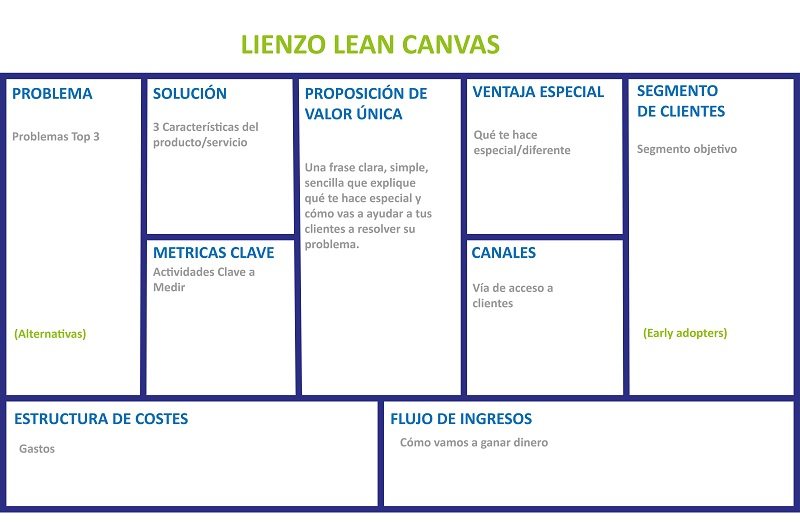
\includegraphics[scale=0.6]{imagenes/leanCanvas.jpg}
\caption{Lean canvas}
\label{leanCanvas}
\end{center}
\end{figure}

Estas hipótesis no conforman el modelo de negocio definivo, si no que irán evolucionando a lo largo de la vida de la empresa de acuerdo al feedback de los clientes. Esta evolución del producto en relación a los deseos del clientes se denomina \textbf{customer development} y es uno de los conceptos claves en Lean startup.

El ciclo de vida de una startup se basa en tres pasos fundamentales que se repiten cíclicamente:
\begin{itemize}
	\item Construir: se diseña el producto en función de las hipótesis que se establecen en el \textbf{lean canvas}. En la primera iteración se crea una versión del producto que tenga las minímas funcionalidades necesarias para aportar valor a los potenciales clientes. Esta versión del producto se denomina \textbf{producto minímo viable}. El objetivo de esta etapa es ''comenzar a recopilar datos y medir resultados. Este modelo de producto no busca ser el resultado final sino un producto suficiente para testar la reacción del potencial cliente" \cite{antevenio2016}.
	\item Medir: tras contrastar nuestras hipótesis de negocio con los clientes a través del \textbf{producto minímo viable} obtenemos información sobre nuestro producto y sobre la propia empresa mediante \textbf{métricas clave}. Dichas métricas (tales como ¿Cuánto cuesta captar un cliente? o ¿Cuánto dinero gastamos mensualmente?) son valoraciones objetivas sobre el rendimiento del producto y de la empresa, y calcularlas de forma periódica es importante ya que permite trazar una evolución y detectar errores y mejoras en la estrategia empresarial.
	\item Aprender: es una etapa clave ya que si el conocimiento obtenido se aplica, se estará más cerca de crear un producto que los clientes quieran comprar. ''este conocimiento adquirido se debe aplicar a un nuevo proceso que comienza de nuevo. Se vuelve a crear un producto, que será una mejora del mismo lo que hace arrancar de nuevo el círculo de crear, medir y aprender" \cite{antevenio2016}. Al llegar a este punto las startups se deben plantear si realizar un pequeño ajuste al producto y volver a \textbf{iterar} o si bien, en caso de que los resultados del producto hayan sido un desastre, hacer cambios de base al modelo de negocio. Estos cambios que afectan a una o más hipótesis del \textbf{lean canvas} se denominan \textbf{pivotar} y consisten en ''cambiar una hipótesis fundamental sobre el producto, la estrategia, y el motor de crecimiento" \cite{emooc}.
\end{itemize}

El proceso se puede realizar cuantas veces sea necesario hasta conseguir el producto que se considere más acorde al cliente. La metodología Lean Startup no trata de evitar que fallemos en el primer intento de lanzar al mercado nuestro servicio, sino que trata de que ese fallo nos salga más ‘barato’ al haber empleado una cantidad considerablemente menor de tiempo y de recursos materiales y económicos \cite{andreapelaez} .






\chapter{Marco Teórico}
\label{marcoteorico}

El contenido de este capítulo es una especie de muestrario de cosas que puedes hacer con \LaTeX.  Por ejemplo, incluir una cita bibliográfica   \cite{BOE_IM_UA} dentro del texto. En esta página de demostración también puedes encontrar información útil acerca de cómo escribir con  \LaTeX.\footnote{En http://metodos.fam.cie.uva.es/~latex/apuntes/apuntes.html hay unos buenos apuntes al respecto.}

Hacer una lista es simple en \LaTeX. Para ello has de crear un entorno (así se llama) itemize con
\begin{verbatim}
\begin{itemize}
...
\end{itemize}
\end{verbatim}
Y dentro de esa estructura, añadir cada elemento de la lista precedido de 
\begin{verbatim}
\item primer item de lista
\item segundo item de lista
...
\item ultimo item de lista
\end{verbatim}
\section{Elaboración de listas.}

Es importante que revises este texto tal como aparece en la plantilla y relaciones el aspecto que tiene el PDF final con cómo está escrito el documento \LaTeX.

Aquí va una lista:
\begin{itemize}
    \item Ingeniería Informática.
    \item Ingeniería Sonido e Imagen en Telecomunicación.
    \item Ingeniería Multimedia.
    \begin{itemize}
         \item Mención: Creación y ocio digital.
         \item Mención: Gestión de Contenidos.
    \end{itemize}
\end{itemize}

Ahora veremos otra estructura más: las tablas.

\section{Inserción de tablas}

Aquí va una tabla\footnote{En http://www.tablesgenerator.com/ se puede encontrar un generador On-Line de tablas para \LaTeX} para que se vea cómo insertar una tabla simple dentro del documento.

\begin{table}[h]
\begin{center}
\begin{tabular}{lllll}
&columna A&columna B&columna C\\
\hline
fila 1&fila 1, columna A & fila 1, columna B & fila 1, columna C\\
fila 2&fila 2, columna A & fila 2, columna B & fila 2, columna C\\
fila 3&fila 3, columna A & fila 3, columna B & fila 3, columna C\\ \hline
\end{tabular}
\end{center}
\caption{Ejemplo de tabla.}
\label{tabladeejemplo}
\end{table}

\LaTeX usa un sistema de parámetros para ``decorar'' las tablas. Puedes consultar estos parámetros en la tabla \ref{tabla_parametros} de la página \pageref{tabla_parametros}. La tabla se ubicará donde, a juicio de \LaTeX, menos moleste por lo que puede no aparecer necesariamente donde se ha insertado en el texto original. 

\begin{table}
\begin{center}
\begin{tabular}{|c|p{0.8\textwidth}|}
\hline
Parámetro & \multicolumn{1}{c|}{Significado} \\ \hline
\texttt{h} & Situa el elemento flotante \emph{preferentemente}
(es decir, si es posible) en la situación exacta donde se incluye este \\
\texttt{t} & Situa el elemento en la parte de arriba de la página \\
\texttt{b} & Situa el elemento en la parte de abajo de la página \\
\texttt{p} & Situa el elemento en una página aparte dedicada sólo a
elementos flotantes; en el caso del formato \texttt{article},
ésta se situa al final del documento, mientras que para al book es
colocada al final de cada capítulo \\ \hline
\end{tabular}
\end{center}
\caption{Parámetros optativos de los entornos flotantes}
\label{tabla_parametros}
\end{table}



\section{Inserción de figuras}

Las figuras son un caso un poco especial ya que \LaTeX busca el mejor lugar para ponerlas, no siendo necesariamente el ligar donde está la referencia. Por ello es importante añadirle un ``caption'' y un ``label'' para poder hacer referencia a ellas en el párrafo correspondiente. Nosotros ponemos la referencia a la figura \ref{logo_im} que está en la página \pageref{logo_im}. justo aquí debajo, pero \LaTeX puede que la ubique en otro lugar.

\begin{figure}
\begin{center}

\includegraphics[scale=0.25]{imagenes/logoim.jpg}
\caption{Logo de Ingeniería  Multimedia.}
\label{logo_im}
\end{center}
\end{figure}

\begin{figure}
\begin{center}

\includegraphics[scale=0.25]{imagenes/logoeps.jpg}
\caption{Logo de la EPS.}
\label{logo_eps}
\end{center}
\end{figure}

\section{Inserción de código}
A veces tendrás que insertar algún pedazo de código fuente para explicar algo relacionado con él. No sustituyas explicaciones con enormes listados de código. Si pones algo de código en tu TFG que sea para demostrar algo o explicar alguna solución.

\LaTeX te ayuda a escribir código de manera que su presentación tenga las marcas y tabulaciones propias de este tipo de texto. Para ello, debes poner el código que escribas DENTRO de un entorno  que se llama ``listings''.  La plantilla ya tiene una serie de instrucciones para incluir el paquete ``listings'' y añadirle algunos modificadores por lo que no tienes que incluirlo tú. Simplemente, mete tu código en el entorno ``lstlisting'' y ya está. Puedes indicar el lenguaje en el que está escrito el código y así \LaTeX lo mostrará mejor. Veamos un ejemplo en la figura \ref{C_code}:

Si pones 
\begin{verbatim}
\begin{lstlisting}[style=C, caption={ejemplo código C},label=C_code]
#include <stdio.h>
int main(int argc, char* argv[]) {
  puts("Hola mundo!");
}
\end{lstlisting}
\end{verbatim}

El resultado será:
\begin{lstlisting}[style=C, caption={ejemplo código C},label=C_code]
#include <stdio.h>
int main(int argc, char* argv[]) {
  puts("Hola mundo!");
}
\end{lstlisting}

Por supuesto, puedes mejorar esta presentación utilizando mas modificadores. Esta información y mucha más puede ser encontrada en \cite{listing_packagge} y en \cite{heinz1listings}.

Otro ejemplo, ahora para mostrar código PHP, sería escribir en tu fichero \LaTeX lo siguiente:
\begin{verbatim}
 \begin{lstlisting}[style=PHP, caption={ejemplo código PHP},label=PHP_code]
 /* 
Ejemplo de código en PHP para escribir tu primer programa en este lenguaje
Copia este código en tu ordenador y ejecútalo
*/
<html>
  <head>
    <title>Prueba de PHP</title>
  </head>
  <body>
    <?php echo '<p>Hola Mundo</p>'; ?> //esto lo escribe TODO el mundo
  </body>
</html>
 \end{lstlisting}
\end{verbatim}
 
 y el resultado es: (ver listado \ref{PHP_code})
 
 \begin{lstlisting}[style=PHP, caption={ejemplo código PHP},label=PHP_code]
/* 
Ejemplo de código en PHP para escribir tu primer programa en este lenguaje. Copia este código en tu ordenador y ejecútalo
*/
 <html>
  <head>
    <title>Prueba de PHP</title>
  </head>
  <body>
    <?php echo '<p>Hola Mundo</p>'; ?> //esto lo escribe TODO el mundo
  </body>
</html>
 \end{lstlisting}
 
 Observa cómo \LaTeX ha puesto los comentarios en gris y ajustado el código para que se muestre más claro.
 
 Si quieres añadir código en otros lenguajes, cambia el comando que dice ``style=nombredellenguaje'' por ``languaje=nombredelnuevolenguaje''.
%input{capitulos/objetivos}
%input{capitulos/metodologia}
%input{capitulos/desarrollo}
%input{capitulos/resultados}
%input{capitulos/conclusiones}


\appendix
\chapter{Anexo I}
Aquí vendría en anexo I 
%\input{glosario/entradas_glosario}
% \addcontentsline{toc}{chapter}{Glosario} %si se usa glosario hay que añadirlo al índice
% \printglossary %muestra el glosario
\printbibliography

\end{document}
